\section{予測の提供と来訪促進システム}
以上のモデルを用いて算出された予測結果は RESTful な Web API で提供され，特定のシステムにこだわらない柔軟な活用を想定している．
予測において十分な精度を確認され，それを活用した来訪促進システムが実装された．


この研究の主題である来訪促進システムは予測機能を外部モジュールとして利用する設計になっており，その前提からこの予測機能にも汎用的な設計が求められている．
特定のシステムやプラットフォームに依存しないため，来訪促進だけでなく混雑の可視化や設備予約支援など他のシステムへの応用も期待される．
Web API としての実装によりインターネット経由で予測結果を取得できるため予測モデルを様々な環境に統合できる．
本研究で提案するシステムも，このようにして提供された予測結果を利用している．


このシステムが提供する Web API ではさまざまなユースケースが想定されて設計されている．
「来訪」「帰宅」といった行動の指定に加えて，ユーザの指定や曜日，行動確率を取得したい時刻などの指定が可能となっている．
全てのリクエストに GET メソッド が採用され，不正なリクエストに対して各種エラーコードを返す構成としている．


% \paragraph{共通の話題に着目した来訪促進システム}
以上で述べた在室予測を用いて，図\ref{fig:DICOMO}のような複数人でのコミュニケーションを促す共通の話題に着目した来訪促進システムが提案されている．
コミュニティ内の共通の話題や関心を持つメンバ同士で形成するグループに対して，人数条件を満たすタイミングを通知し活動の活性化を狙っている．
具体的にはコミュニティ内の全ユーザにおいて23:59までに来訪する確率が閾値を超えるメンバの行動の発生予測時刻を用いて，活動の成立が期待される時間帯を抽出している．
既存のチャットツール上で動作する Bot 型の拡張アプリケーションとして実装され，翌日の予定検討に影響を与えられる時間帯に通知を送信している．

\begin{figure}[htb]
  \centering
  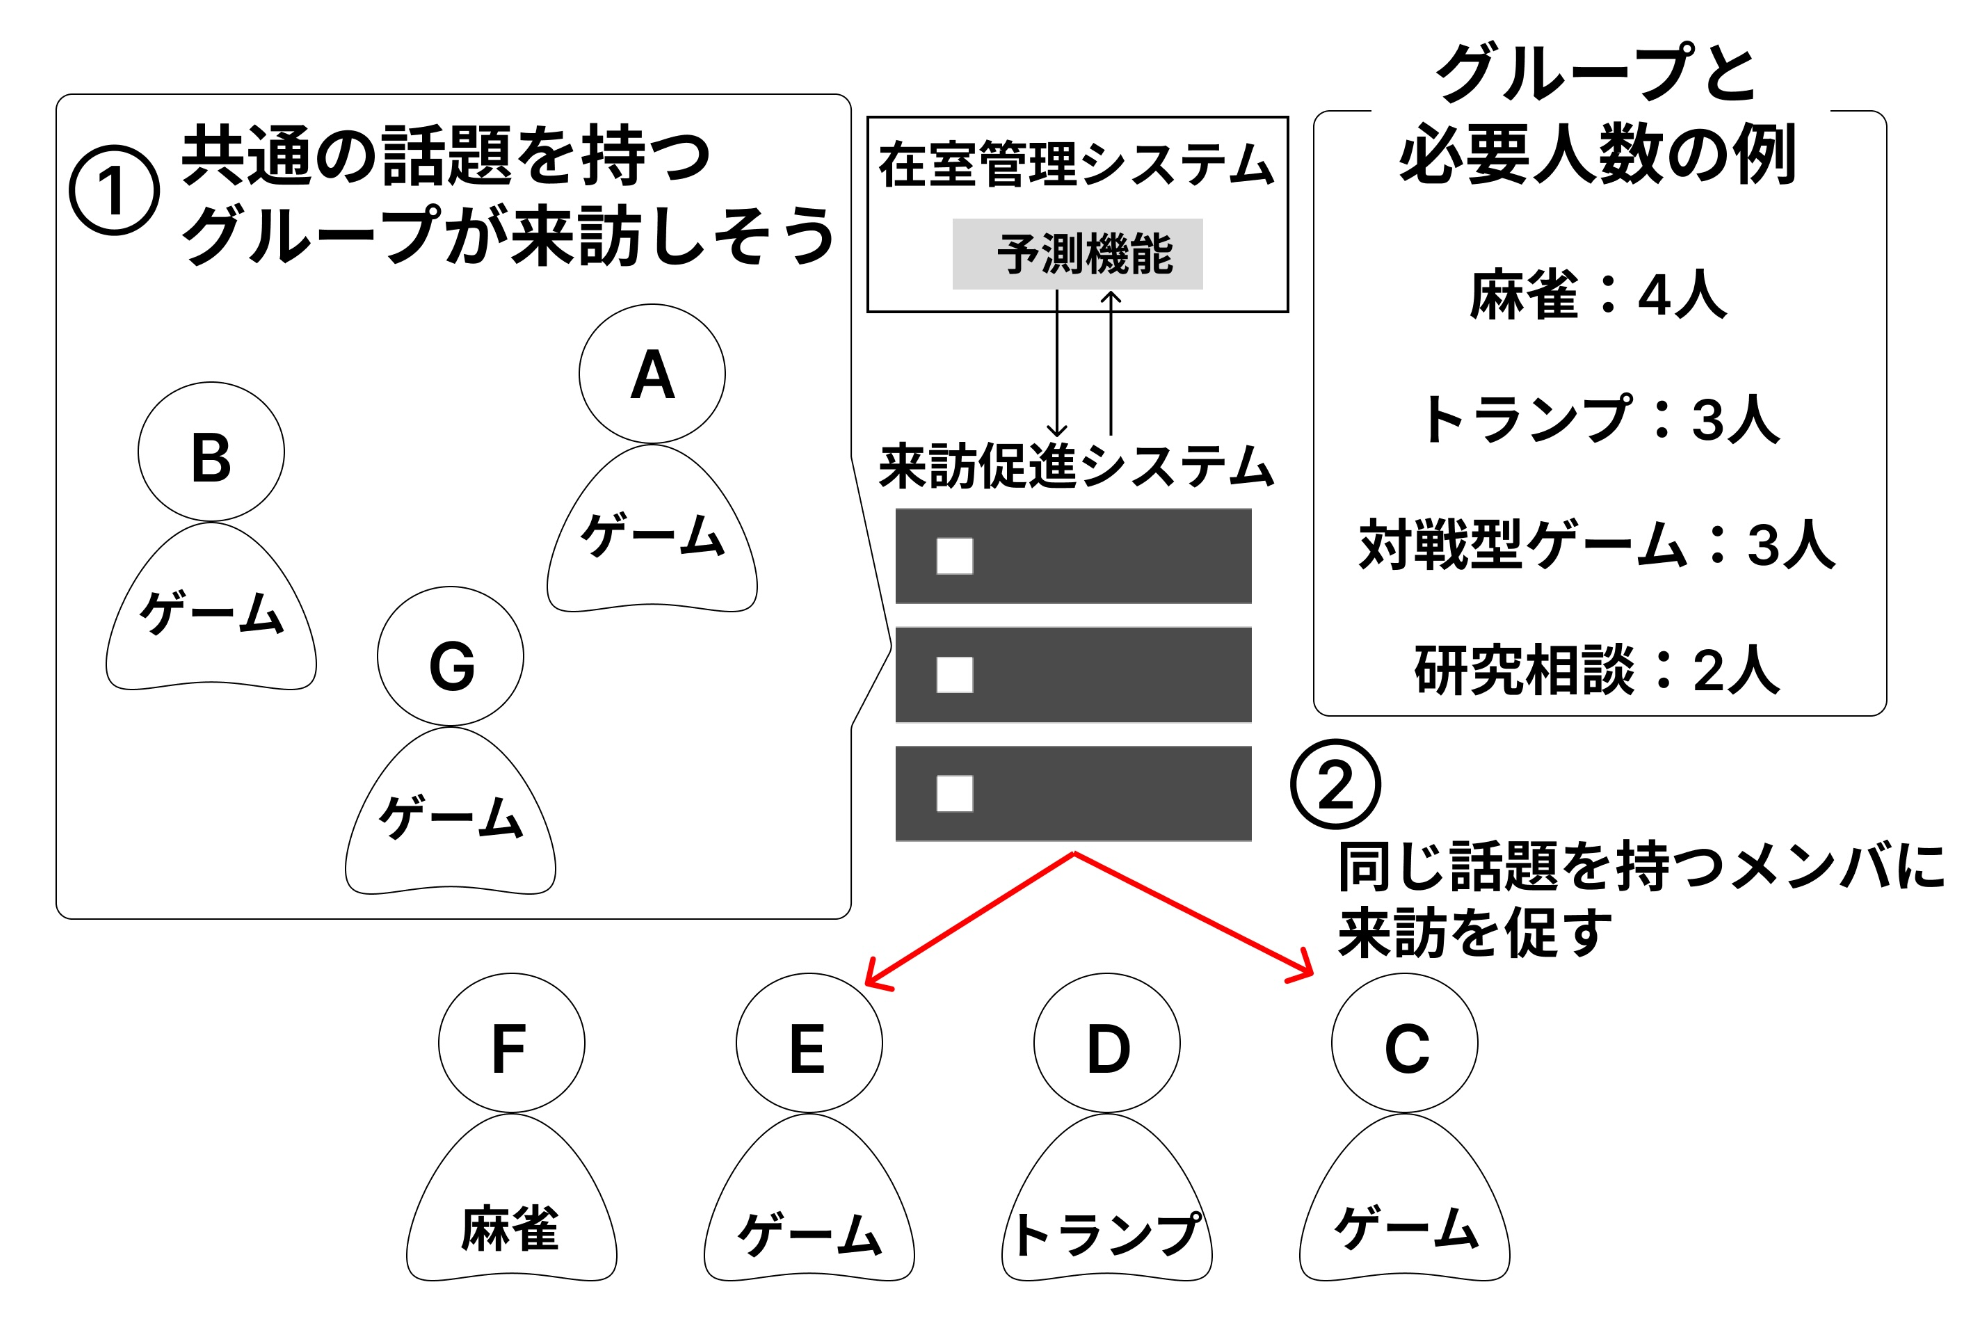
\includegraphics[width=0.8\linewidth]{fig/DICOMO.png} % suzuki
  \caption{来訪促進システムの概要(文献\cite{hayashi}より引用)}
  \label{fig:DICOMO}

\end{figure}